\documentclass[12pt]{article}

%%%%%%%%%%%%%%%%%%%%%%%%%%%%%%%%%%%%%%%%%%%%%%%%%%%%%%%%%%%%%%%%%%%%%%%%%%%%%%%%
%                           Package preset for homework
%%%%%%%%%%%%%%%%%%%%%%%%%%%%%%%%%%%%%%%%%%%%%%%%%%%%%%%%%%%%%%%%%%%%%%%%%%%%%%%%
% Miscellaneous
\usepackage[margin=1in]{geometry}
\usepackage[utf8]{inputenc}
\usepackage{indentfirst}
\usepackage{blindtext}
\usepackage{graphicx}
\usepackage{xr-hyper}
\usepackage{hyperref}
\usepackage{enumitem}
\usepackage{color}
\usepackage{float}
% Math
\usepackage{latexsym}
\usepackage{amsfonts}
\usepackage{amssymb}
\usepackage{amsmath}
\usepackage{commath}
\usepackage{amsthm}
\usepackage{bbold}
\usepackage{bm}
% Physics
\usepackage{physics}
\usepackage{siunitx}
% Code typesetting
\usepackage{listings}
% Citation
\usepackage[authoryear]{natbib}
\usepackage{appendix}
\usepackage[capitalize]{cleveref}
% Title & name
\title{Homework}
\author{Tien Vo}
\date{\today}


%%%%%%%%%%%%%%%%%%%%%%%%%%%%%%%%%%%%%%%%%%%%%%%%%%%%%%%%%%%%%%%%%%%%%%%%%%%%%%%%
%                   User-defined commands and environments
%%%%%%%%%%%%%%%%%%%%%%%%%%%%%%%%%%%%%%%%%%%%%%%%%%%%%%%%%%%%%%%%%%%%%%%%%%%%%%%%
%%% Misc
\sisetup{load-configurations=abbreviations}
\newcommand{\due}[1]{\date{Due: #1}}
\newcommand{\hint}{\textit{Hint}}
\let\oldt\t
\renewcommand{\t}[1]{\text{#1}}

%%% Bold sets & abbrv
\newcommand{\N}{\mathbb{N}}
\newcommand{\Z}{\mathbb{Z}}
\newcommand{\R}{\mathbb{R}}
\newcommand{\Q}{\mathbb{Q}}
\let\oldP\P
\renewcommand{\P}{\mathbb{P}}
\newcommand{\LL}{\mathcal{L}}
\newcommand{\FF}{\mathcal{F}}
\newcommand{\HH}{\mathcal{H}}
\newcommand{\NN}{\mathcal{N}}
\newcommand{\ZZ}{\mathcal{Z}}
\newcommand{\RN}[1]{\textup{\uppercase\expandafter{\romannumeral#1}}}
\newcommand{\ua}{\uparrow}
\newcommand{\da}{\downarrow}

%%% Unit vectors
\newcommand{\xhat}{\vb{\hat{x}}}
\newcommand{\yhat}{\vb{\hat{y}}}
\newcommand{\zhat}{\vb{\hat{z}}}
\newcommand{\nhat}{\vb{\hat{n}}}
\newcommand{\rhat}{\vb{\hat{r}}}
\newcommand{\phihat}{\bm{\hat{\phi}}}
\newcommand{\thetahat}{\bm{\hat{\theta}}}

%%% Other math stuff
\providecommand{\units}[1]{\,\ensuremath{\mathrm{#1}}\xspace}
% Set new style for problem
\newtheoremstyle{problemstyle}  % <name>
        {10pt}                   % <space above>
        {10pt}                   % <space below>
        {\normalfont}           % <body font>
        {}                      % <indent amount}
        {\bfseries\itshape}     % <theorem head font>
        {\normalfont\bfseries:} % <punctuation after theorem head>
        {.5em}                  % <space after theorem head>
        {}                      % <theorem head spec (can be left empty, 
                                % meaning `normal')>

% Set problem environment
\theoremstyle{problemstyle}
\newtheorem{problemenv}{Problem}[section]
\newenvironment{problem}[1]{%
  \renewcommand\theproblemenv{#1}%
  \problemenv
}{\endproblemenv}
% Set lemma environment
\newenvironment{lemma}[2][Lemma]{\begin{trivlist}
\item[\hskip \labelsep {\bfseries #1}\hskip \labelsep {\bfseries #2.}]}{\end{trivlist}}
% Set solution environment
\newenvironment{solution}{
    \begin{proof}[Solution]$ $\par\nobreak\ignorespaces
}{\end{proof}}
\numberwithin{equation}{problemenv}

%%% Page format
\setlength{\parindent}{0.5cm}
\setlength{\oddsidemargin}{0in}
\setlength{\textwidth}{6.5in}
\setlength{\textheight}{8.8in}
\setlength{\topmargin}{0in}
\setlength{\headheight}{18pt}

%%% Code environments
\definecolor{dkgreen}{rgb}{0,0.6,0}
\definecolor{gray}{rgb}{0.5,0.5,0.5}
\definecolor{mauve}{rgb}{0.58,0,0.82}
\lstset{frame=tb,
  language=Python,
  aboveskip=3mm,
  belowskip=3mm,
  showstringspaces=false,
  columns=flexible,
  basicstyle={\small\ttfamily},
  numbers=none,
  numberstyle=\tiny\color{gray},
  keywordstyle=\color{blue},
  commentstyle=\color{dkgreen},
  stringstyle=\color{mauve},
  breaklines=true,
  breakatwhitespace=true,
  tabsize=4
}
\lstset{
  language=Mathematica,
  numbers=left,
  numberstyle=\tiny\color{gray},
  numbersep=5pt,
  breaklines=true,
  captionpos={t},
  frame={lines},
  rulecolor=\color{black},
  framerule=0.5pt,
  columns=flexible,
  tabsize=2
}


\title{Homework 3: Phys 7320 (Spring 2022)}
\due{February 2, 2022}

\begin{document}
\maketitle
%%%%%%%%%%%%%%%%%%%%%%%%%%%%%%%%%%%%%%%%%%%%%%%%%%%%%%%%%%%%%%%%%%%%%%%%%%%%%%%
\begin{problem}{1}[Scattering for a perfectly conducting sphere]
In class we discussed scattering off a dielectric sphere; now we consider the
case of a perfectly conducting sphere of radius $a$. Jackson discusses this in
Sec. 10.1.C so we will fill in the details.

When the radiation hits the target, it induces both an electric dipole moment
$\vb{p}$ and a magnetic dipole moment $\vb{m}$, which in Gaussian units take the
form,
\begin{equation}
    \vb{p}=a^3\vb{E}_\text{inc},\qquad
    \vb{m}=-\frac{a^3}{2}\vb{B}_\text{inc}
\end{equation}
or for SI units, see Jackson (10.12)--(10.13).

(a) Show why this leads to the differential scattering cross section given in
Jackson (10.14) (in either unit system).

(b) Calculate the results for scattering for polarization both parallel and
perpendicular to the plane of scattering, as in Jackson (10.15). Include the
factor $1/2$ so that when they are added together in part (c), you are
calculating the total cross section averaged over initial polarizations.

(c) Caculate the total differential cross-section averaged over polarizations
(10.16) and the polarization $\Pi(\theta)$ (10.17). Is radiation more likely to
continue in a forward direction, or to be scattered backwards? Is radiation more
likely to be scattered parallel to, or perpendicular to, the plane of
scattering? Compare these behaviors to the case of scattering from a
dielectric sphere.
\begin{solution}
(a) Given
\begin{equation}
    \vb{p}
    =4\pi\epsilon_0a^3\vb{E}_\text{inc}
    =4\pi\epsilon_0a^3E_0e^{ik\vb{n}_0\vdot\vb{x}}\bm\epsilon_0 
\end{equation}
and
\begin{equation}
    \vb{m}
    =-2\pi a^3\vb{H}_\text{inc}
    =-2\pi a^3\sqrt{\epsilon_0/\mu_0}\vb{n}_0\times\vb{E}_\text{inc}  
    =-2\pi a^3\sqrt{\epsilon_0/\mu_0}E_0e^{ik\vb{n}_0\vdot\vb{x}}\vb{n}_0\times
    \bm\epsilon_0,
\end{equation}
we can plug into (10.4, Jackson) and calculate
\begin{align}
    \frac{d\sigma}{d\Omega}
    &=\frac{k^4}{(4\pi\epsilon_0 E_0)^2}
    \abs{\bm\epsilon^\ast\vdot\vb{p}+\frac1c(\vb{n}\times\bm\epsilon^\ast)\vdot\vb{m}}^2\notag\\
    &=k^4a^6\abs{\bm\epsilon^\ast\vdot\bm\epsilon_0
    +\qty(\vb{n}\times\bm\epsilon^\ast)\vdot\qty[\frac{-2\pi\sqrt{\epsilon_0/\mu_0}}{4\pi\epsilon_0c}(\vb{n}_0\times\bm\epsilon_0)]}^2\notag\\
    &=k^4a^6\abs{\bm\epsilon^\ast\vdot\bm\epsilon_0
    -\frac12\qty(\vb{n}\times\bm\epsilon^\ast)\vdot\qty(\vb{n}_0\times\bm\epsilon_0)}^2
\end{align}

(b) Let $\vb{n}_0=\zhat$ and $\vb{n}=\sin\theta\xhat+\cos\theta\zhat$ so that
$\vb{n}\vdot\vb{n}_0=\cos\theta$. Then, in the perpendicular case,
$\bm\epsilon=\yhat$ and $\bm\epsilon_0=\pm\yhat$. We can then calculate
\begin{align}
    \qty(\vb{n}\times\bm\epsilon^\ast)\vdot\qty(\vb{n}_0\times\bm\epsilon_0)
    =\qty(\sin\theta\zhat-\cos\theta\xhat)\vdot\qty(\mp\xhat)
    =\pm\cos\theta 
\end{align}
and $\bm\epsilon^\ast\vdot\bm\epsilon_0=\pm 1$. It follows, then, that
\begin{equation}
    \abs{\bm\epsilon^\ast\vdot\bm\epsilon_0-\frac12\qty(\vb{n}\times\bm\epsilon^\ast)\vdot\qty(\vb{n}_0\times\bm\epsilon_0)}^2=
    \abs{(\pm 1)\qty(1-\frac12\cos\theta)}^2=\abs{1-\frac12\cos\theta}^2
\end{equation}
Thus, when averaged over the two possible initial polarizations, we get
\begin{equation}
    \frac{d\sigma_\bot}{d\Omega}=\frac{k^4a^6}{2}\abs{1-\frac12\cos\theta}^2 
\end{equation}

Similarly, in the parallel case, $\bm\epsilon=\cos\theta\xhat-\sin\theta\yhat$
(so that $\bm\epsilon\vdot\vb{n}=0$) and $\bm\epsilon_0=\pm\xhat$ (so that
$\bm\epsilon_0\vdot\vb{n}_0=0$). We can calculate
$\bm\epsilon^\ast\vdot\bm\epsilon_0=\pm\cos\theta$ and
\begin{equation}
    (n\times\bm\epsilon^\ast)\vdot\qty(\vb{n}_0\times\bm\epsilon_0)
    =\qty(\sin^2\theta\yhat+\cos^2\theta\yhat)\vdot\qty(\pm\yhat)
    =\pm1
\end{equation}
Thus,
\begin{equation}
    \abs{\bm\epsilon^\ast\vdot\bm\epsilon_0-\frac12\qty(\vb{n}\times\bm\epsilon^\ast)\vdot\qty(\vb{n}_0\times\bm\epsilon_0)}^2
    =\abs{(\pm1)\qty(\cos\theta-\frac12)}^2=\abs{\cos\theta-\frac12}^2
\end{equation}
Thus, averaging over the polarizations,
\begin{equation}
    \frac{d\sigma_\parallel}{d\Omega}
    =\frac{k^4a^6}{2}\abs{\cos\theta-\frac12}^2
\end{equation}

(c) The total differential cross section is
\begin{align}
    \frac{d\sigma}{d\Omega}=\frac{d\sigma_\bot}{d\Omega}+\frac{d\sigma_\parallel}{d\Omega}=
    &=\frac{k^4a^6}{2}\qty[\qty(\cos\theta-\frac12)^2+\qty(1-\frac12\cos\theta)^2]\notag\\
    &=\frac{k^4a^6}{2}\qty(\frac54\cos^2\theta-2\cos\theta+\frac54)\notag\\
    &=k^4a^6\qty[\frac58(1+\cos^2\theta)-\cos\theta]
\end{align}
and the polarization is
\begin{align}
    \Pi(\theta)
    =\frac{d\sigma_\bot/d\Omega-d\sigma_\|/d\Omega}{d\sigma/d\Omega}
    =\frac{(3/8)k^4a^6}{k^4a^6[(5/8)(1+\cos^2\theta)-\cos\theta]}
    =\frac{3}{5\cos^2\theta-8\cos\theta+5}
\end{align}
A plot for $\Pi$ is included below. Since the peak is at
$\theta\approx40^\circ$, the radiation is more likely to be scattered parallel
to the plane of scattering. This is different from the case of scattering from a
dielectric sphere (peak at $\theta_\bot=90^\circ$)
\begin{center}
    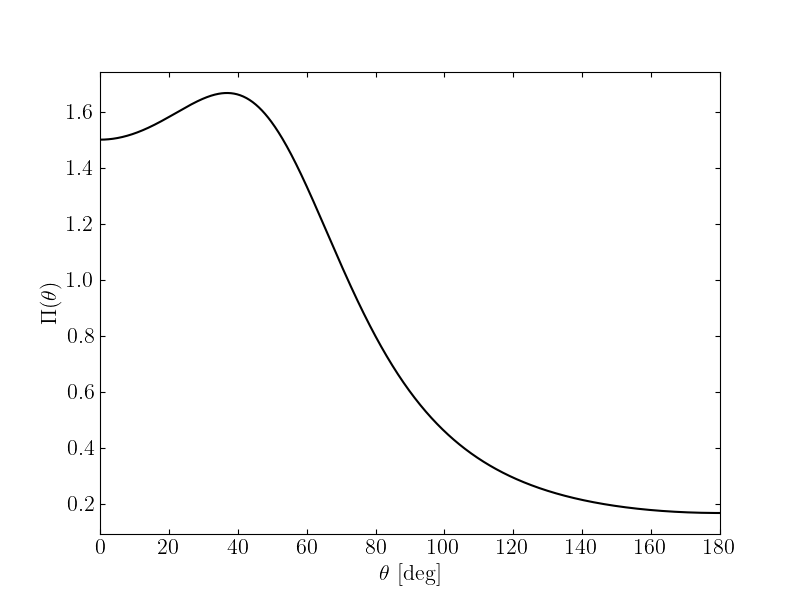
\includegraphics[width=0.7\textwidth]{p1c.png}
\end{center}
\end{solution}
\end{problem}
\newpage
%%%%%%%%%%%%%%%%%%%%%%%%%%%%%%%%%%%%%%%%%%%%%%%%%%%%%%%%%%%%%%%%%%%%%%%%%%%%%%%    
%%%%%%%%%%%%%%%%%%%%%%%%%%%%%%%%%%%%%%%%%%%%%%%%%%%%%%%%%%%%%%%%%%%%%%%%%%%%%%%
\begin{problem}{2}[Power scattered and power absorbed]
An unpolarized wave of frequency $\omega=ck$ is scattered by a \textit{slightly}
lossy uniform isotropic dielectric sphere of radius $R$ much smaller than a
wavelength. The sphere is characterized by an ordinary real dielectric constant
$\epsilon_r$ and a real conductivity $\sigma$. The parameters are such that the
skin depth $\delta$ is very \textit{large} compared to the radius $R$.

(a) Calculate the differential and total \textit{scattering} cross sections.

(b) Show that the absorption cross section is
\begin{equation}
    \sigma_\text{abs}=12\pi
    R^2\frac{RZ_0\sigma}{(\epsilon_r+2)^2+(Z_0\sigma/k)^2} 
\end{equation}

\begin{solution}
(a) In the long wavelength approximation, we can use the results for a dielectric
sphere in uniform electromagnetic fields. From (10.5, Jackson), the dipole 
moment is
\begin{equation}
    \vb{p}
    =4\pi\epsilon_0E_0R^3\frac{\epsilon/\epsilon_0-1}{\epsilon/\epsilon_0+2}\bm\epsilon_0e^{ik\vb{n}_0\vdot\vb{x}}
    =4\pi\epsilon_0E_0R^3\frac{\epsilon_r-1+i\sigma/\omega}{\epsilon_r+2+i\sigma/\omega}\bm\epsilon_0e^{ik\vb{n}_0\vdot\vb{x}}
\end{equation}
Thus, the differential cross section is
\begin{align}
    \frac{d\sigma}{d\Omega}
    &=\frac{k^4}{(4\pi\epsilon_0E_0)^2}\abs{\bm\epsilon^\ast\vdot\vb{p}}^2\notag\\
    &=k^4R^6\abs{\frac{\epsilon_r-1+i\sigma/\omega}{\epsilon_r+2+i\sigma/\omega}}^2\abs{\bm\epsilon^\ast\vdot\bm\epsilon_0}^2\notag\\
    &=k^4R^6\frac{(\epsilon_r-1)^2+\sigma^2/\omega^2}{(\epsilon_r+2)^2+\sigma^2/\omega^2}\abs{\bm\epsilon^\ast\vdot\bm\epsilon_0}^2
\end{align}
An unpolarized wave contains all polarizations. So averaging over all
polarizations gives
\begin{equation}
    \frac{d\sigma}{d\Omega}=\frac{k^4R^6}{2}\frac{(\epsilon-1)^2+\sigma^2/\omega^2}{(\epsilon_r+2)^2+\sigma^2/\omega^2}(1+\cos^2\theta) 
\end{equation}
and the total scattering cross section is
\begin{equation}
    \sigma=\pi
    k^4R^6\frac{(\epsilon_r-1)^2+\sigma^2/\omega^2}{(\epsilon_r+2)^2+\sigma^2/\omega^2}\int_0^\pi(1+\cos^2\theta)\sin\theta
    d\theta
    =\frac{8\pi}{3}k^4R^6\frac{(\epsilon_r-1)^2+\sigma^2/\omega^2}{(\epsilon_r+2)^2+\sigma^2/\omega^2}
\end{equation}
\end{solution}
\end{problem}
\newpage
%%%%%%%%%%%%%%%%%%%%%%%%%%%%%%%%%%%%%%%%%%%%%%%%%%%%%%%%%%%%%%%%%%%%%%%%%%%%%%%
%%%%%%%%%%%%%%%%%%%%%%%%%%%%%%%%%%%%%%%%%%%%%%%%%%%%%%%%%%%%%%%%%%%%%%%%%%%%%%%
\begin{problem}{3}[An atom in a spring]
Suppose you model the atom as an electron on a spring of natural frequency
$\omega_0$. Include a damping force $\vb{F}=-\Gamma d\vb{x}/dt$. Put the spring
in an external electric field $\vb{E}e^{-i\omega t}$, solve for the steady state
motion, compute the resulting dipole moment, and drop the result into the
appropriate formula for the differential cross section. Now do physics: note how
you recover Rayleigh scattering for $\omega\ll\omega_0$. At high frequency, the
cross section becomes independent of frequency. This is called the Thomson cross
section. (It is the same formula for scattering off a free electron). There is a
dimensionful constant
\begin{equation}
    r_0=\frac{e^2}{m_ec^2} 
\end{equation}
where $m_e$ is the electron mass, which characterizes the scale of elastic light
scattering on electrons and hence on atoms. Find a number for this in cm. This
says that the natural scale for light scattering on the electrons in atoms is
$\sigma\sim r_0^2$ (or maybe more correctly, $r_0^2(\omega/\omega_0)^4$, which
is even smaller). Notice how all the interesting polarization behavior is
frequency-independent. This isn't true when you work in complete generality, but
it is true in dipole approximation. There are other ways to derive this result
which we'll encounter later on in the course.
\begin{solution}
By Newton's second law, the equation of motion is
\begin{equation}\label{p3:eom}
    \frac{d^2\vb{x}}{dt^2}
    =-\omega_0^2\vb{x}-\frac{\Gamma}{m}\frac{d\vb{x}}{dt}
    -\frac{e}{m}\vb{E}e^{-i\omega t}
\end{equation}
The steady state solution is oscillatory. Thus, suppose a solution is
$\vb{x}=\vb{A}e^{-i\omega t}$. Then, plugging back into \eqref{p3:eom}, we get
\begin{equation}
    -\omega^2\vb{A}=-\omega_0^2\vb{A}+i\frac{\Gamma\omega}{m}\vb{A}-\frac{e}{m}\vb{E} 
    \Rightarrow\vb{A}=\frac{e}{m}\frac{1}{\omega^2-\omega_0^2+i\Gamma\omega/m}\vb{E}
\end{equation}
Thus, the full solution is
\begin{equation}
    \vb{x}=\frac{e}{m}\frac1{\omega^2-\omega_0^2+i\Gamma\omega/m}\vb{E}e^{-i\omega
    t} 
\end{equation}
The dipole moment is then
\begin{equation}
    \vb{p}=-e\vb{x}
    =-\frac{e^2}{m}\frac1{\omega^2-\omega_0^2+i\Gamma\omega/m}\vb{E}
    e^{-i\omega t}
\end{equation}
Letting $\vb{E}=E_0\bm\epsilon_0$, we can calculate the differential cross
section from (10.4, Jackson),
\begin{align}
    \frac{d\sigma}{d\Omega}
    &=\frac{k^4}{(4\pi\epsilon_0E_0)^2}\abs{\bm\epsilon^\ast\vdot\vb{p}}^2\notag\\
    &=\frac{k^4e^4}{m^2(4\pi\epsilon_0)^2}\abs{\frac1{\omega^2-\omega_0^2+i\Gamma\omega/m}\bm\epsilon^\ast\vdot\bm\epsilon_0}^2\notag\\
    &=\frac{c^4k^4r_0^2}{(\omega^2-\omega_0^2)^2+\Gamma^2\omega^2/m^2}\abs{\bm\epsilon^\ast\vdot\bm\epsilon_0}^2
\end{align}
Averaging over all polarizations ($\perp$ and $\parallel$), we get the final 
result
\begin{equation}
    \frac{d\sigma}{d\Omega}=\frac{c^4k^4r_0^2}{(\omega^2-\omega_0^2)^2+\Gamma^2\omega^2/m^2}\frac{1+\cos^2\theta}{2} 
\end{equation}
For $\omega\ll\omega_0$, the denominator is $\sim\omega_0^4$ and
$d\sigma/d\Omega$ scales as $k^4$, in accordance with Rayleigh scattering. For
$\omega\gg\omega_0$, the denominator is $\sim\omega^4$, but $ck/\omega=1$, so
\begin{equation}
    \frac{d\sigma_\text{Thomson}}{d\Omega}=\frac12r_0^2(1+\cos^2\theta)
\end{equation}
is indeed independent of $\omega$, where
\begin{equation}
    r_0=\frac1{4\pi\epsilon_0}\frac{e^2}{mc^2} 
    \approx2.82\times10^{-13}\,\unit{cm}
\end{equation}
So the total cross section $\sigma$ scales as $r_0^2$.
\end{solution}
\end{problem}
%%%%%%%%%%%%%%%%%%%%%%%%%%%%%%%%%%%%%%%%%%%%%%%%%%%%%%%%%%%%%%%%%%%%%%%%%%%%%%%
\end{document}
